% Enable warnings about problematic code
\RequirePackage[l2tabu, orthodox]{nag}

\documentclass{WeSTassignment}

% The lecture title, e.g. "Web Information Retrieval".
\lecture{Introduction to Web Science}
% The names of the lecturer and the instructor(s)
\author{%
  Prof. Dr.~Steffen~Staab\\{\normalsize\mailto{staab@uni-koblenz.de}} \and
  Ren{\'e}~Pickhardt\\{\normalsize\mailto{rpickhardt@uni-koblenz.de}} \and
   Korok~Sengupta\\{\normalsize\mailto{koroksengupta@uni-koblenz.de}} \and 
   Olga~Zagovora\\{\normalsize\mailto{zagovora@uni-koblenz.de}}
}
% Assignment number.
\assignmentnumber{8}
% Institute of lecture.
\institute{%
  Institute of Web Science and Technologies\\%
  Department of Computer Science\\%
  University of Koblenz-Landau%
}
% Date until students should submit their solutions.
\datesubmission{January 11, 2017, 10:00 a.m.}
% Date on which the assignments will be discussed in the tutorial.
\datetutorial{January 13, 2017, 12:00 p.m.}

% Set langauge of text.
\setdefaultlanguage[
  variant = american, % Use American instead of Britsh English.
]{english}

% Specify bib file location.
\addbibresource{bibliography.bib}

% For left aligned centerd boxes
% see http://tex.stackexchange.com/a/25591/75225
\usepackage{varwidth}
\usepackage{minted} %nice package for highliting lprogramming code
% ==============================================================================
% Document

\begin{document}

\maketitle
Please look at all the lessons of part 2 in particular \textbf{Similarity of Text} and \textbf{graph based models}

For all the assignment questions that require you to write code, make sure to include the code in the answer sheet, along with a separate python file. Where screen shots are required, please add them in the answers directly and not as separate files.\\ \\ 

Other than that this sheet is mainly designed to review and apply what you have learnt in part 2 it is a little bit larger but there is also more time over the x-mas break. In any case we wish you a mery x-mas and a happy new year. 

%Please mention your team Names here: 
Team Name: XXXX


\section{Similarity - (40 Points)}
This assignment will have one exercise which is dived into four subparts. 
The main idea is to study once again the web crawl of the Simple English Wikipedia. The goal is also to review and aply your knowledge from part 2 of this course.

We have constructed two data sets from it which are all the articles and the link graph extracted from Simple English Wikipedia. The extracted data sets are stored in the file \url{http://141.26.208.82/store.zip} which contains a pandas container and can be read with pandas in python. In subsection ``1.5 Hints"  you will find some sample python code that demonstrates how to easily access the data.

With this data set you will create three different models with different similarity measures and finally try to evaluate how similar these models are. 

\textbf{This assignment requires you to handle your data in efficient data structures otherwise you might discover runtime issues. So please read and understand the full assignment sheet with all the tasks that are required before you start implementing some of the tasks.}

\subsection{Similarity of Text documents  (10 Points)}
\subsubsection{Jaccard - Similarity on sets}
\begin{enumerate}
\item Build the word sets of each article for each article id.
\item Implement a function \texttt{calcJaccardSimilarity(wordset1, wordset2)} that can calculate the jaccard coefficent of two word sets and return the value.
\item Compute the result for the articles \texttt{Germany} and \texttt{Europe}.
\end{enumerate}

\subsubsection{TF-IDF with cosine similarity}
\begin{enumerate}
\item Count the term frequency of each term for each article
\item Count the document frequencies of each term. 
\item For each article id provide a dictionary of terms occuring in the article together with their tf-idf scores as the corresponding values.
\item Implement a function \texttt{calculateCosineSimilarity(tfIdfDict1, tfIdfDict2)} that computes the cosine similarity for two sparse tf-idf vectors and returns the value.
\item Compute the result for the articles \texttt{Germany} and \texttt{Europe}.
\end{enumerate}

\subsection{Similarity of Graphs (10 Points)}
You can understand the similarity of two articles by comparing their sets of outlinks (and see how much they have in common). Feel free to reuse the \texttt{computeJaccardSimilarity} function from the first part of the exercise. This time do not aply it on the set of words within two articles but rather on the set of outlinks being used within two articles. Again compute the result for the articles \texttt{Germany} and \texttt{Europe}.

\subsection{How similar have our similarities been? (10 Points)}
Having implemented these three models and similarity measures (text with Jaccard, text with cosine, graph with Jaccard) our goal is to understand and quantify what is going on if they are used in the wild. Therefore in this and the next subtask we want to try to give an answere to the following questions.

\begin{itemize}
\item Will the most similar articles to a certain article always be the same independent which model we use?
\item How similar are these measures to each other? How can you statistically compare them?
\end{itemize}

Assume you could use the similarity measure to compute the top k most similar articles for each article in the document collection. We want to analyze how different the rankings for these various models are. 

Do some research to find a statistical measure (either from the lectures of part 2 or by doing a web search and coming up with something that we haven't discussed yet) that could be used best to compare various rankings for the same object. 

Explain in a short text which measure you would use in such an experiment and why you think it is usefull for our task. 

\subsection{Implement the measure and do the experiment (10 Points)}
After you came up with a measure you will most likely run into another problem when you plan to do the experiment. 

Since runtime is an issue we cannot compute the similarity for all pairs of articles. Tell us: 
\begin{enumerate}
\item How many similarity computations would have to be done if you wished to do so? 
\item How much time would roughly be consumed to do all of these computations?
\end{enumerate}

A better strategy might be to select a couple of articles for which you could compute your meassure. One strategy would be to select the 100 longest articles. Another strategy might be to randomly select 100 articles from our corpus. 

Computer your three similarity measures and evaluate them for these two strategies of selecting test data. Present your results. Will the results depend on the method for selecting articles? What are your findings?

\textbf{Answer:}
\textbf{Code:}
\lstinputlisting{similarity.py}
\textbf{Word Rank Frequency Diagram:}\\
\hspace*{-100px}
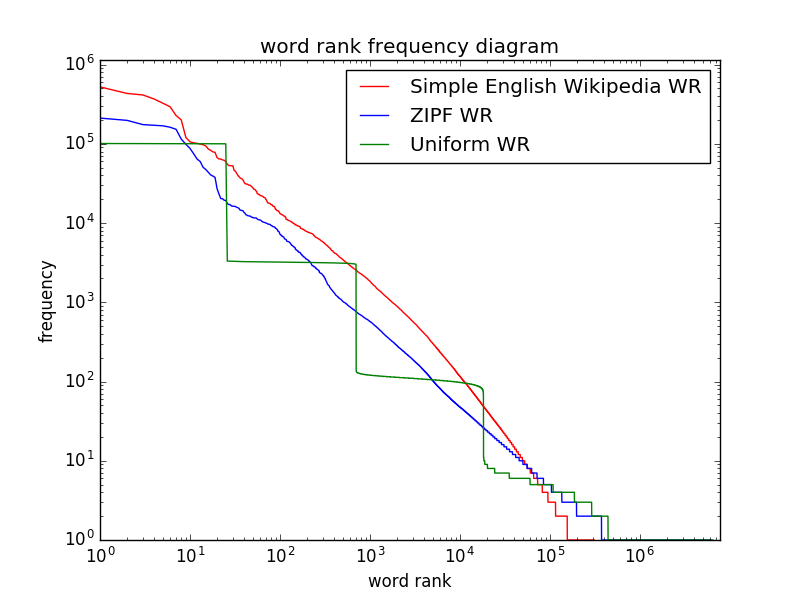
\includegraphics[width=600px]{../task2/wrfd}

\textbf{Answer to 1.3:} \\
The most similar articles to a certain article will be different, depending on which model is used. The reason for this is because the Jaccard Similarity only checks the occurrence of a term in two documents. The amount of occurrences, however, is not being considerd.\\
The Cosine Similarity on the other hand takes these occurrences into account and the similarity rating decreases, the more often the word occurres in a document.
This would lead to different similarity rankings, because the Jaccard Similarity would rank documents with many filler terms higher than the Cosine Similarity, where the rating of those filler terms should be quite low due to the common usage.\\
One could measure the rankings by setting up a query to a certain subject, as for example a famous person in a certain field, and check if information about this person / subject is ranked higher than information not related to the person / subject. As an example, we take a famous musician and set up a query. The top k most similar articles should be about the person himself, his band, if any, other musicians who play the same instrument or other musicians who played with him.


\subsection{Hints:}
\begin{enumerate}
\item In oder to access the data in python, you can use the following pice of code:
\begin{minted}[]{python} 
import pandas as pd
store = pd.HDFStore('store.h5')
df1=store['df1'] 
df2=store['df2'] 
\end{minted}
\item Variables df1 and df2 are pandas DataFrames which is tabular data structure. df1 consists of article's texts, df2 represents links from Simple English Wikipedia articles. Variables have the following columns:
\begin{itemize}
\item ``name" is a name of Simple English Wikipedia article,
\item ``text" is a full text of the article ``name",
\item ``out\_links" is a list of article names where the article ``name" links to.
\end{itemize}
\item In general you might want to store the counted results in a file before you do the similarity computations and all the research for the third and fourth subtask. Doing all this counting and preperation might allready take quite some runtime. 
\item When computing the sparse tf-idf vectors you might allready want to store the eukleadan length of the vectors. otherwise you might discover runtime issues when computing the length again for each similarity computation. 
\item Finding the top similar articles for a given article id requires you to compute the similarity of the given article with comparison to all the other known articles and extract the top 5 similarities. Bare in mind that these are quite a lot of similarity computations! You can expect a runtime to find the top similar articles with respect to one of the methods to be up to 10 seconds. If it takes significant longer then you probably have not used the best data structures handle your data.
\item \textbf{Even though many third party libraries exist to do this task with even less computational effort those libraries must not be used.}
\item You can find more information about basic usage of pandas DataFrame in  \href{http://pandas.pydata.org/pandas-docs/stable/dsintro.html#column-selection-addition-deletion}{pandas documentation}.
\item Here are some usefull examples of operations with DataFrame:
\begin{minted}[]{python} 
import pandas as pd

store = pd.HDFStore('store.h5')#read .h5 file
df1=store['df1'] 
df2=store['df2'] 
print df1['name'] # select column "name"
print df1.name # select column "name"
print df1.loc[9] #select row with id equals 9 
print df1[5:10] #select rows from 6th to 9th (first row is 0) 
print df2.loc[0].out_links #select outlinks of article with id=0 

#show all columns where column "name" equals "Germany"
print df2[df2.name=="Germany"]

#show column out_links for rows where name is from list ["Germany","Austria"]
print df2[df2.name.isin(["Germany","Austria"])].out_links 

#show all columns where column "text" contains word "good" 
print df1[df1.text.str.contains("good")]

#add word "city" to the beginning of each text value 
#(IT IS ONLY SHOWS RESULT OF OPERATION, see explanation below!)
print df1.text.apply(lambda x: "city "+x)

#make all text lower case and split text by spaces
df1[["text"]]=df1.text.str.lower().str.split()

def do_sth(x):
	#here is your function
	#
	#
	return x
    
#apply do_sth function to text column 
#Iit will not change column itself, it will only show the result of aplication	 	
print df1.text.apply(do_sth())

#you always have to assign result to , e.g., column, 
#in order it affects your data.
#Some functions indeed can change the DataFrame by 
#applying them with argument inplace=True
df1[["text"]]=df1.text.apply(do_sth())  

#delete column "text"
df1.drop('text', axis=1, inplace=True)
\end{minted}

\end{enumerate}







\makefooter

\end{document}
